\documentclass[prl,twocolumn,floatfix]{revtex4-2}

\usepackage{graphicx}
\usepackage{bm}

\usepackage{amsmath}
\usepackage{units}

\usepackage{hyperref}
\hypersetup{colorlinks=true, citecolor=blue, urlcolor=blue, linkcolor=blue}

\usepackage{todonotes}

\renewcommand{\vec}[1]{\boldsymbol{#1}}

\begin{document}
\title{Improved imaging of magnetic domains with a photoelectron emission microscope\todo{Improve title?}}

\author{F. O. Schumann}
\email{Electronic mail: schumann@mpi-halle.de}
\affiliation{ Max-Planck-Institut f\"{u}r Mikrostrukturphysik, Weinberg 2, 06120 Halle, Germany}

\author{M. Paleschke}
\author{J. Henk}
\author{W. Widdra}
\affiliation{Institute of Physics, Martin Luther University Halle-Wittenberg, D-06099 Halle (Saale), Germany}

\author{C.-T. Chiang}
\affiliation{Institute of Atomic and Molecular Sciences, Academia Sinica, Taipei, Taiwan}

\date{\today}

\begin{abstract}
Here comes the abstract \ldots
\end{abstract}

\pacs{}

\maketitle

% Paragraph headings may be deleted in the final version
\paragraph{Introduction.} Ultrafast spin and magnetization dynamics is a rapidly growing field in condensed matter physics with promising implications for future research and device applications.  This field includes ultrafast switching and imaging of magnetic domains. Magnetic domain imaging commonly employs X-ray magnetic circular dichroism (XMCD) analyzed with a photoelectron emission microscope (PEEM). The intensity recorded for a particular domain changes with the helicity of the incident core-level resonant radiation, producing magnetic contrast. A spin resolution is not necessary. \todo[inline]{we could give examples for the importance of XMCD} The excitation by circular-polarized X-rays requires typically tunable synchrotron radiation which introduces temporal pulses with widths in the range of tens of picoseconds. The latter renders XMCD-PEEM unsuitable for ultrafast imaging of magnetic domains with femtosecond time resolution. Replacing the synchrotron radiation source by a femtosecond laser allows for experiments in the laboratory and, more importantly, for high time resolution in the order of femtoseconds. Determined by the photon energy, the photoelectrons are excited to energies slightly above the escape threshold, i.e.,to a few tenths of an electronvolt above the vacuum level.  

Early threshold PEEM studies revealed that the magnetic contrast is rather small and therefore might not be sufficient for ultrafast imaging.  \todo[inline]{Add reference}.. on Ni/Cu(001) \todo[inline]{Give number}

The above calls for improving threshold-PEEM while keeping the advantages of a laser-based experiment. In this paper we report on such a refinement of threshold PEEM, in which the magnetic contrast is significantly enhanced. The main idea is to utilize darkfield MCD in threshold photoemission. Momentum and energy selection \ldots 

We apply the new approach to magnetic domains of Fe(100). It is rationalized by symmetry considerations, and the experimental results are supported by state-of-the-art photoemission calculations. In our opinion, this approach is an essential step toward ultrafast imaging of magnetic domains.

\paragraph{Conceptual basis.} Key to the proposed approach are asymmetries of the photoemission intensities, which follow from  symmetry consideration. Since a PEEM detects photoelectrons with (almost) all emission angles, one is concerned with a chiral geometry for photoelectrons with off-normal wavevector $\vec{k}$ (Fig.~\ref{fig:symmetry}). This chirality results in magnetic dichroism and, hence, in magnetic contrast.

\begin{figure}
    \centering
    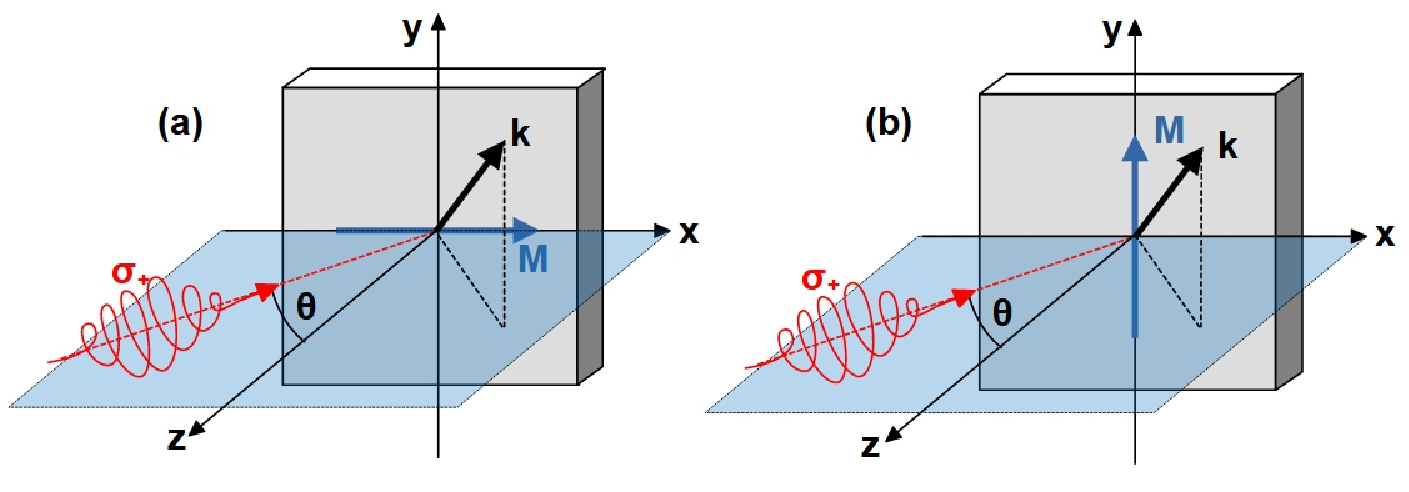
\includegraphics[width = \columnwidth]{symmetry}
    \caption{Symmetry analysis. A circular polarized laser pulse (orange, with helicity $\sigma_{+}$ impinges onto a magnetic domain (rectangular solid, with magnetization direction $\vec{M}$). The pulse's incidence direction and the surface normal ($z$-axis) span the scattering plane (blue; $xz$-plane). The off-normal detection of photoelectrons with wavevector $\vec{k}$ results in a chiral setup. If the scattering plane is a mirror plane of the latiice, the photoemission intensities for fixed $\vec{k}$ obey $I(\sigma_{+}, +\vec{M}) = I(\sigma_{-}, -\vec{M})$ (panel~a) or $I(\sigma_{+}, +\vec{M}) = I(\sigma_{-}, +\vec{M})$ (panel~b).}
    \label{fig:symmetry}
\end{figure}

The photoemission intensity of electrons detected with wavevector $\vec{k}$ depends on the two helicities $\sigma_{\pm}$ of the incident circular polarized laser radiation and on the two orientations $\pm M$ of the in-plane magnetization in a selected domain, yielding four intensities $I_{\vec{k}}(\sigma_{\pm}, \pm M)$ (shortened $I_{\pm \pm}$). The latter are combined into the total intensity
\begin{align}
    I & \equiv I_{+ +} + I_{+ -} + I_{- +} + I_{- -}. 
\end{align}
In order to disentangle the two main contrast mechanisms we define appropriate asymmetries:
\begin{subequations}
\begin{align}
    A_{\mathrm{pol}} & \equiv \left[ \left( I_{+ +} + I_{+ -} \right) - \left( I_{- +} + I_{- -} \right) \right] / I,
    \label{eq:Apol}
    \\
    A_{\mathrm{ex}} & \equiv \left[ \left( I_{+ +} + I_{- -} \right) - \left( I_{+ -} + I_{- +} \right) \right] / I.
    \label{eq:Aex}
\end{align}    
\end{subequations}
In the polarization asymmetry $A_{\mathrm{pol}}$ the magnetization's orientation is averaged out; it thus encodes contrast due to the light's helicity (as if the domain were nonmagnetic). Contrast due to the exchange splitting is quantified by the exchange asymmetry $A_{\mathrm{ex}}$, in which one averages over the mutual orientations of helicity and magnetization.

\paragraph{Experimental aspects.} Setup \ldots

The experimental results as well the conceptual ideas are supported by relativistic photoemission computations, briefly described in the Supplemental Material~\cite{Supplement}.

\paragraph{Contrast mechanisms.} In a first step we analyze the two main contrast mechanism: light polarization and exchange splitting.

The polarization asymmetry $A_{\mathrm{pol}}$, defined in Eq.~\eqref{eq:Apol} and depicted in Fig.~\ref{fig:Apol}, depends on the binding energy of the initial states. Both theoretical (top row) and experimental data (bottom row) show
that this contrast mechanism is sizable (with absolute values up to about $\unit[40]{\%}$ in theory and $\unit[20]{\%}$ in experiment) and thus cannot be ignored. 

\begin{figure*}
    \centering
    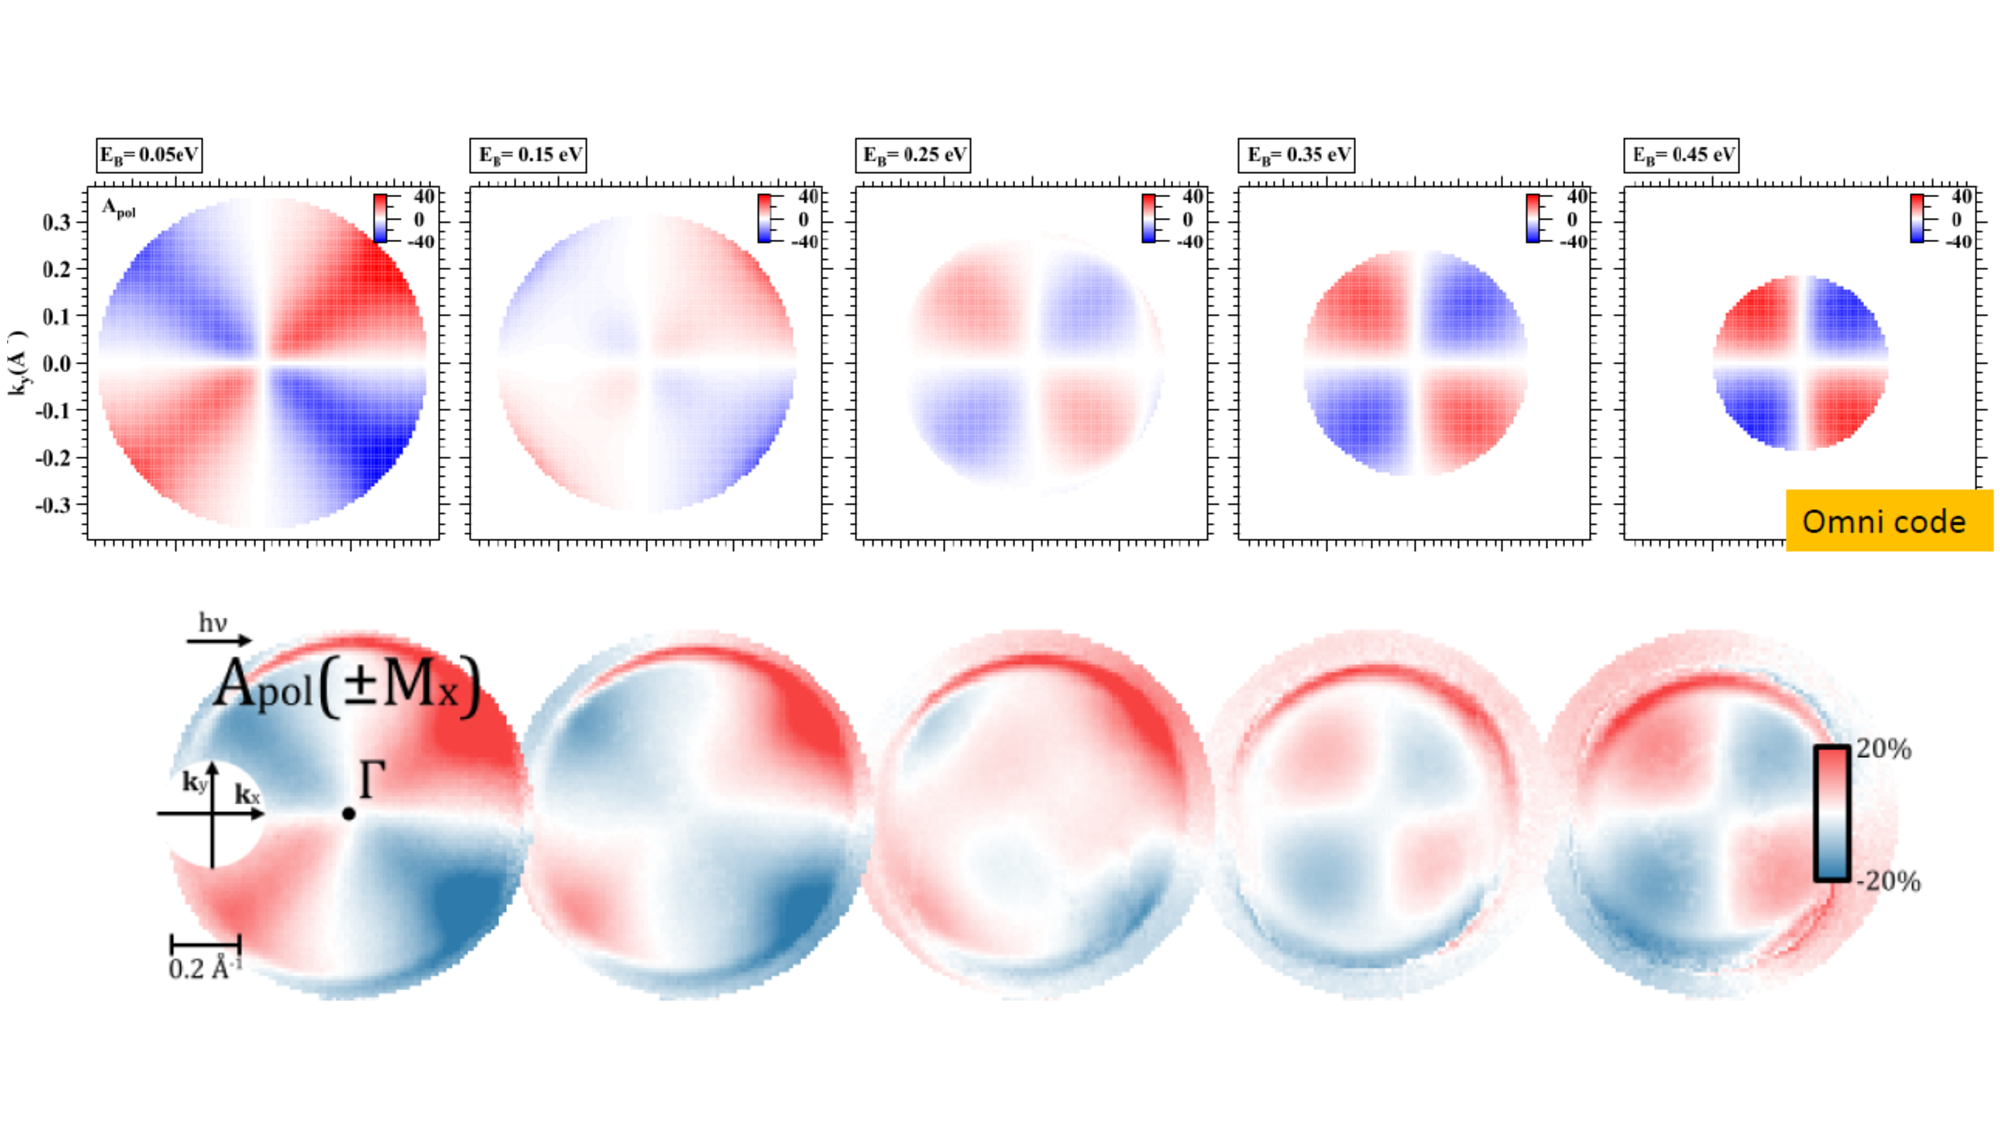
\includegraphics[width = 0.9\textwidth]{Apol}
    \caption{Polarization asymmetry $A_{\mathrm{pol}}$ of Fe(001) at selected binding energies versus wave vector $\vec{k}_{\parallel}$ of the photoelectrons. Top row: theoretical results obtained from photoemission calculations. The binding energy is indicated at each panel. The color scale, showing $A_{\mathrm{pol}}$ as defined in Eq.~\eqref{eq:Apol} in percent, is identical for all panels in this row. Bottom row: respective experimental results. The arrow marked $h \nu$ indicates the light incidence direction. $\Gamma$ is the center of the surface Brillouin zone ($\vec{k}_{\parallel} = $).}
    \label{fig:Apol}
\end{figure*}

The theoretical patterns (top row in Fig.~\ref{fig:Apol}) exhibit two nodal lines ($k_{x} = 0$ and $k_{y} = 0$). Moreover, one finds changes of sign if either $k_{x}$ or $k_{y}$ is reversed. These features are imposed by the symmetry of the setup. The experimental counterparts (bottom row) display the same features but slightly oblique or off-center, most clearly for binding energies with comparably small asymmetry (cf.\ $\unit[0.15]{eV}$ and $\unit[0.25]{eV}$). We attribute these deviations to imperfections in experiment, for example a small misalignment of the light incidence with respect to a crystal mirror plane and inhomogeneous magnetization in the surface layers. Moreover, we assume an electron self-energy that is independent of $k_{\parallel}$ (see \cite{Supplement}). Nevertheless, the agreement of experiment and theory shows that \ldots \todo{More here}

The energy-dependent exchange asymmetry $A_{\mathrm{ex}}$, defined in Eq.~\eqref{eq:Aex} and shown in Fig.~\ref{fig:Aex}, is smaller than $A_{\mathrm{pol}}$ (Fig.~\ref{fig:Apol}) (with absolute values up to $\unit[10]{\%}$ in theory and $\unit[6]{\%}$ in experiment). Nevertheless it exhibits a clear odd symmetry upon reversal of $k_{x}$; it does not change sign upon reversal of $k_{y}$, in contrast to $A_{\mathrm{pol}}$. Both features are dictated by the symmetry of the setup (see \cite{Supplement}).

\begin{figure*}
    \centering
    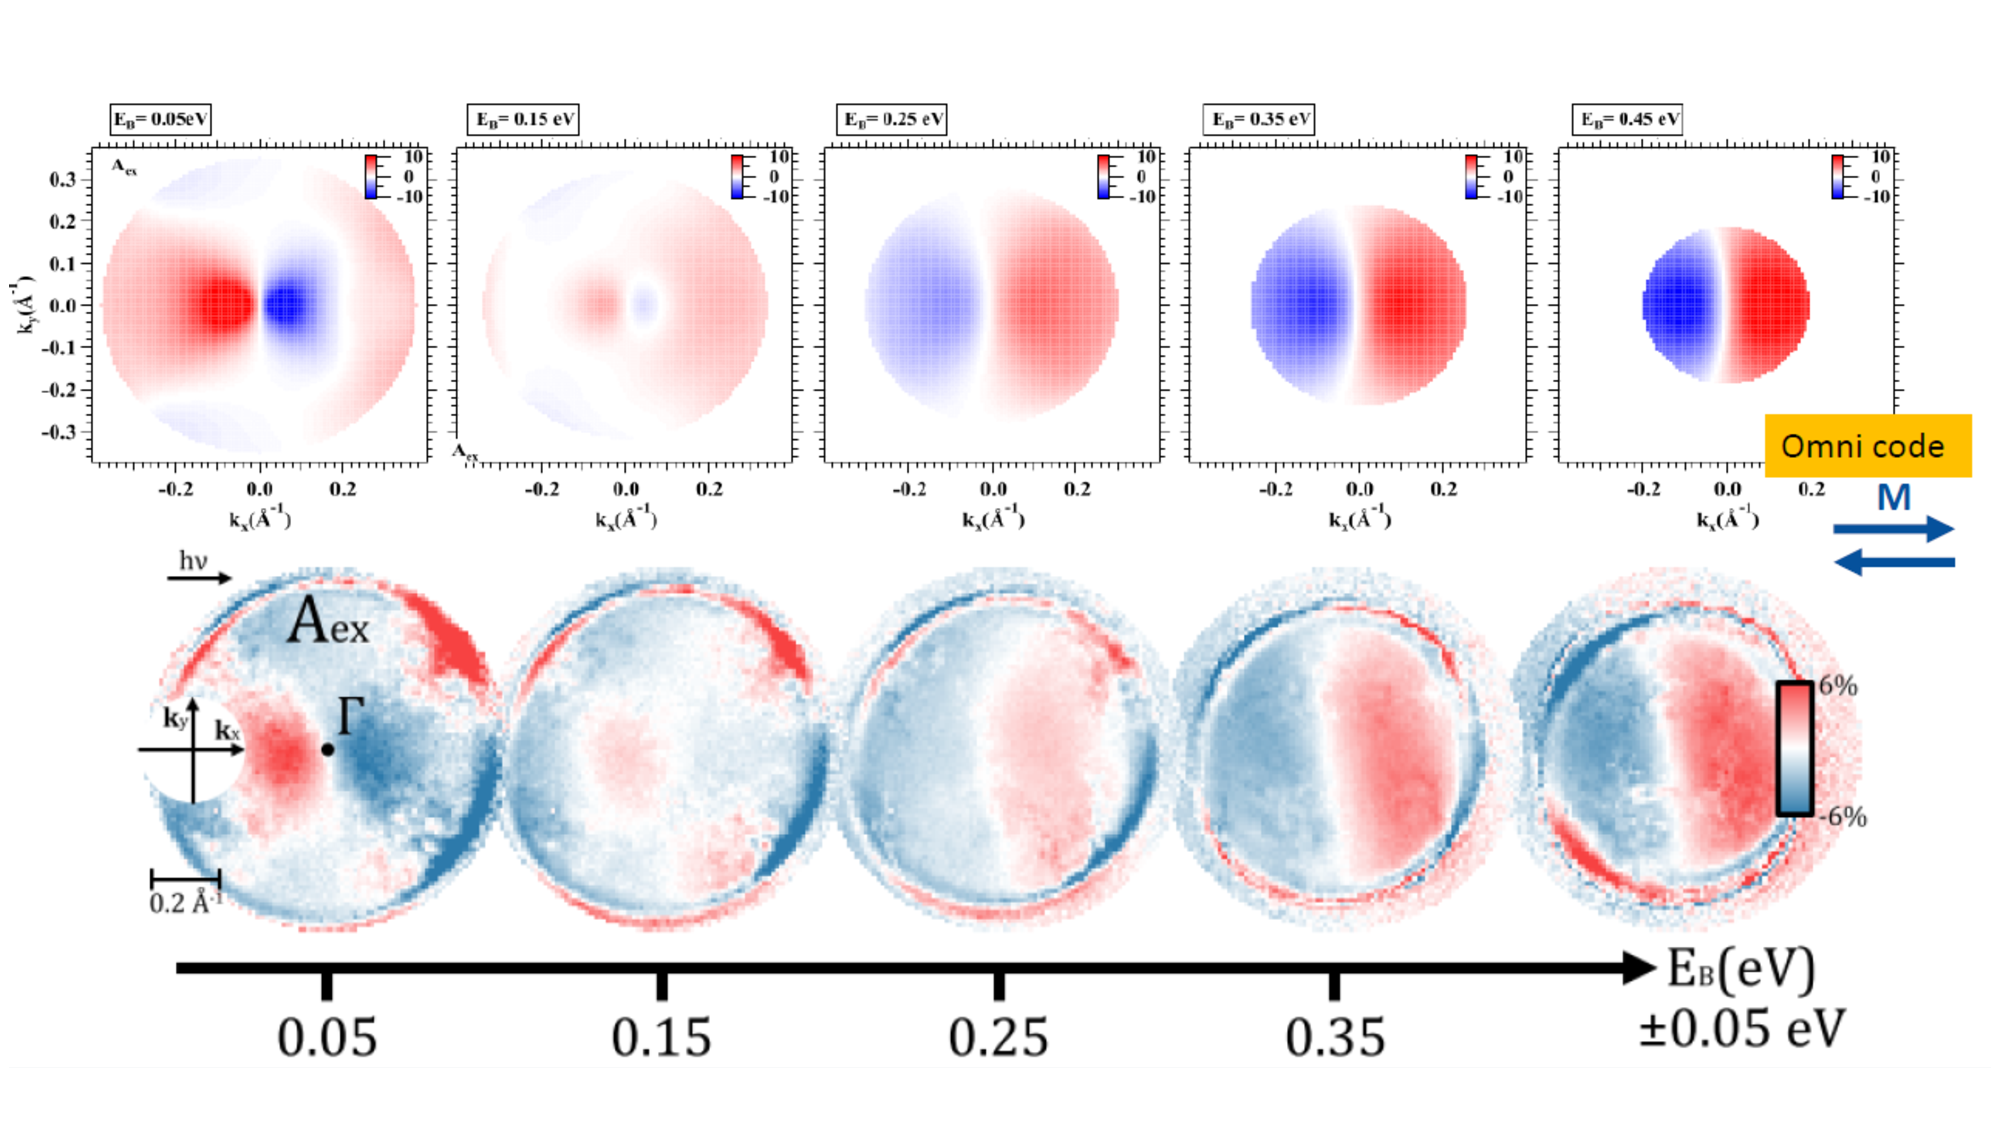
\includegraphics[width = 0.9\textwidth]{Aex}
    \caption{As Figure~\ref{fig:Apol}, but for the exchange asymmetry $A_{\mathrm{ex}}$ of Fe(001). The orientations of the magnetization are indicated by arrows on the right-hand side.}
    \label{fig:Aex}
\end{figure*}

The above findings support that the asymmetries $A_{\mathrm{pol}}$ and $A_{\mathrm{ex}}$ are suitable tools to disentangle and to quantify the main contrast mechanisms for domain imaging. 

\paragraph{Domain imaging.} Aperture, selection of wave vectors.

Center position of the aperture shows very weak contrast (Fig.~\ref{fig:Imaging}).

\begin{figure}
    \centering
    %\includegraphics{}
    \caption{Darkfield magnetic-circular dichroism imaging of Fe(100). Left: schematic, nine aperture positions \ldots. Right: domain imaging using the nine aperture positions.}
    \label{fig:Imaging}
\end{figure}

Sizable contrast in the other off-center positions of the aperture. Allows to image domain structure unequivocally. Size of contrast/asymmetry \ldots

\paragraph{Prospects.} The present investigation proves that magnetic domains can be imaged with a laser-equipped photoelectron emission microscope with high contrast using a momentum-selection of the detected photoelectrons. The common belief that a such PEEM provides only weak contrast is thereby refuted.

For a proof of principle we applied the proposed improvement to in-plane magnetized Fe(001) surfaces. However, the approach is general so that it can easily be applied to other ferromagnets, even to those with out-of-plane magnetization. Thus, it well suited for studying magnetic reorientation transitions, as for example observed for Ni/Cu(001) \todo{Add reference}. We see its main capabilities in investigations of ultrafast magnetization dynamics using femtosecond laser pulses. As applications one might think of ultrafast motion of domain walls \todo{Mention racetrack?} or of large skyrmions.

\paragraph{Acknowledgments.} This work is funded by the Deutsche Forschungsgemeinschaft (DFG, German Research Foundation) -- Project-ID 328545488 -- TRR~227, projects~A06 and~B04.

% \bibliographystyle{}
\bibliography{references}

\listoftodos

\end{document}
